\chapter{Design}\label{chapter:design}
This chapter deals with the algorithms specifically designed for the tangram generator. Before going into detail about these algorithms the overall structure of the application and its interface will be presented. 

Once the user enters the site, the application starts to first pre-compute some values that are repeatedly used throughout the entire program, like direction vectors for tangrams, and then randomly generate tangrams using an algorithm described in section \ref{generate}. As this takes some time depending on the device and the number of tangrams generated, a progress bar indicates the current state of the generation progress. At all time some information about how to interact with the application is displayed below the main interface. In the very beginning this also includes some information about tangrams in general. After the generation progress has finished the tangrams are sorted according to an interestingness measure and the 6 top ranked tangrams are displayed for the user to choose from. An option for generating new tangrams is also provided. Some candidates for interestingness measures are presented in section \ref{interesting}. If the user clicks on one of the displayed shapes, a bigger version of the tangram becomes visible and he or she can attempt to solve the puzzle by translating, rotating and flipping the puzzle pieces until they cover the whole given shape. At this point it is also possible to simply display the solution or receive a hint showing the position of one of the tans. 
In order to collect some statistics about which tangrams are preferred and how they are solved, some data is send to a database and can then be used to derive new interesting measures. Each time the user chooses one of 6 tangrams, his choice along with 6 tangrams. Statistics sent after solving a puzzle include the tangram itself as well as the time needed to solve the puzzle, the number of hints used and the number of actions performed to reach a solution.

The final user interface is shown in Figures \ref{choose} and \ref{game}.

\begin{figure}
\centering
    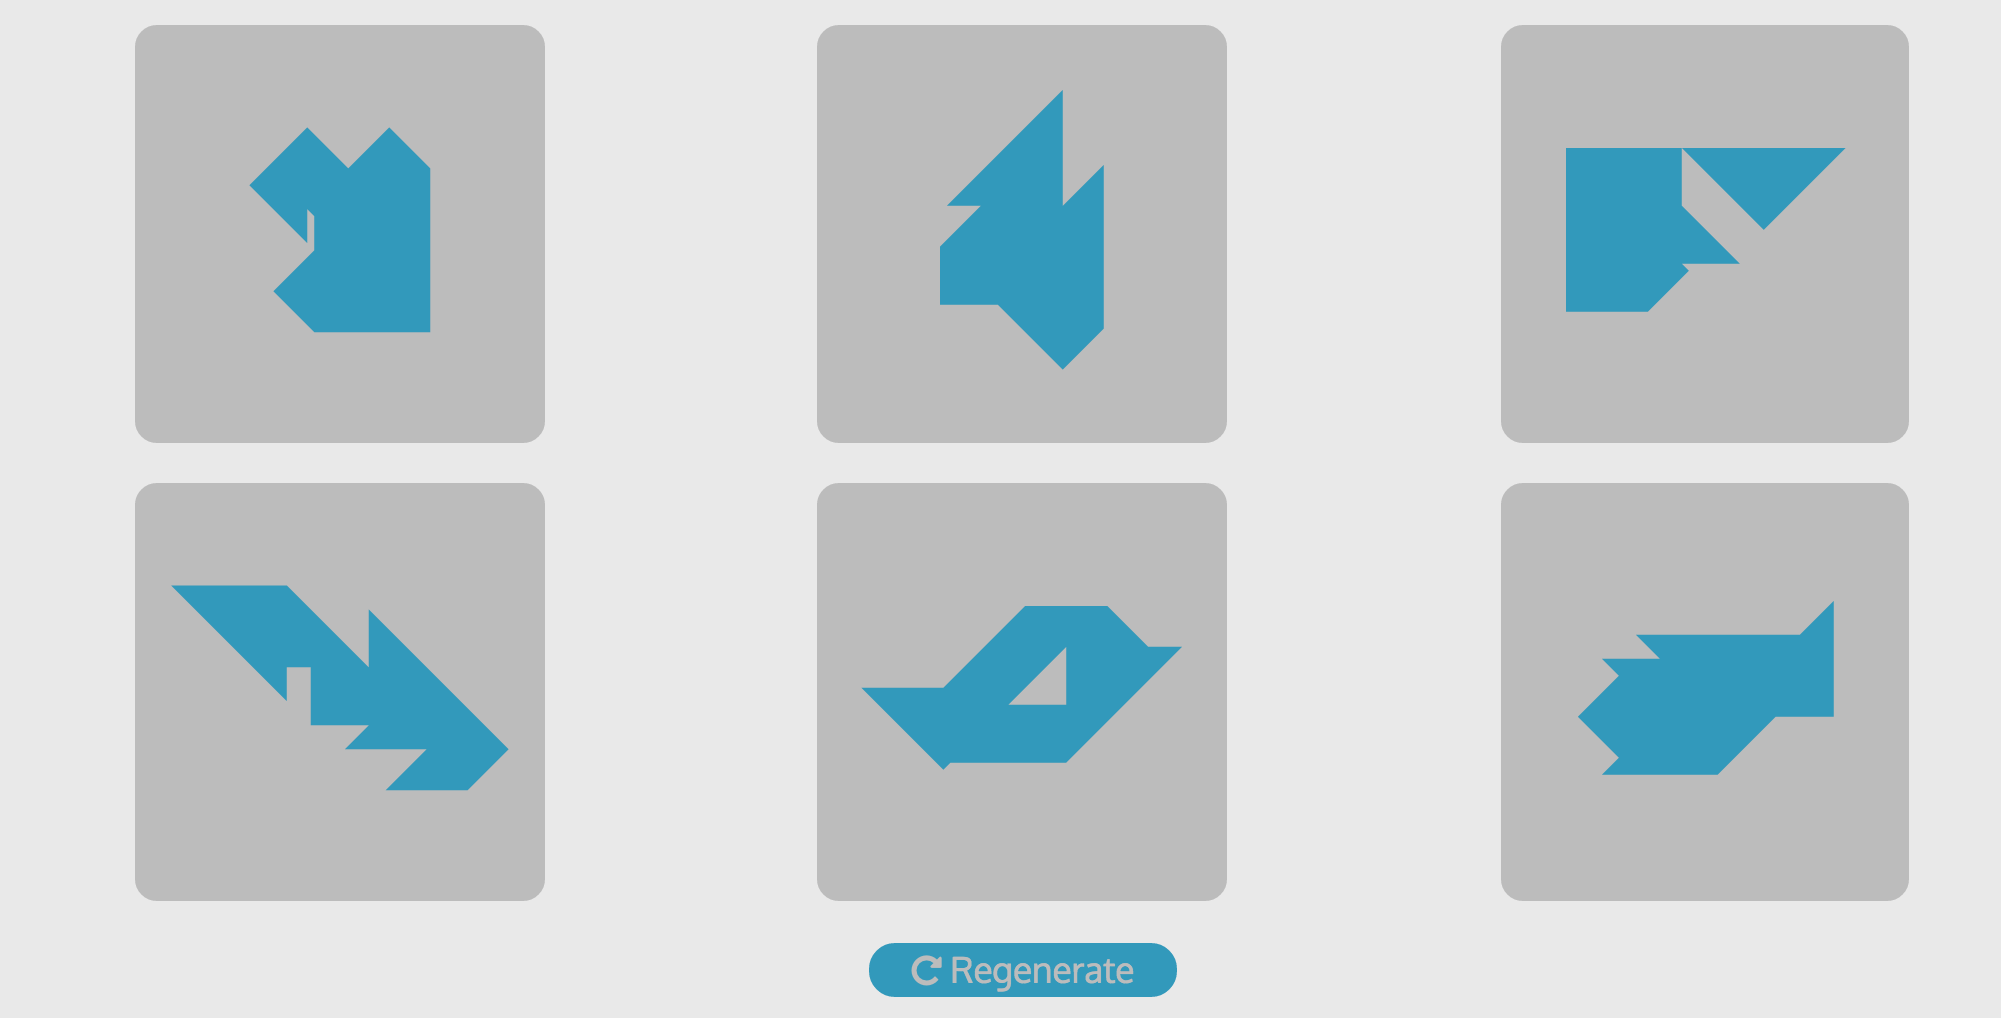
\includegraphics[width=0.9\textwidth]{figures/chose.png}
\caption{Interface showing 6 tangrams to the user to choose from}
\label{choose}
\end{figure}

\begin{figure}
\centering
    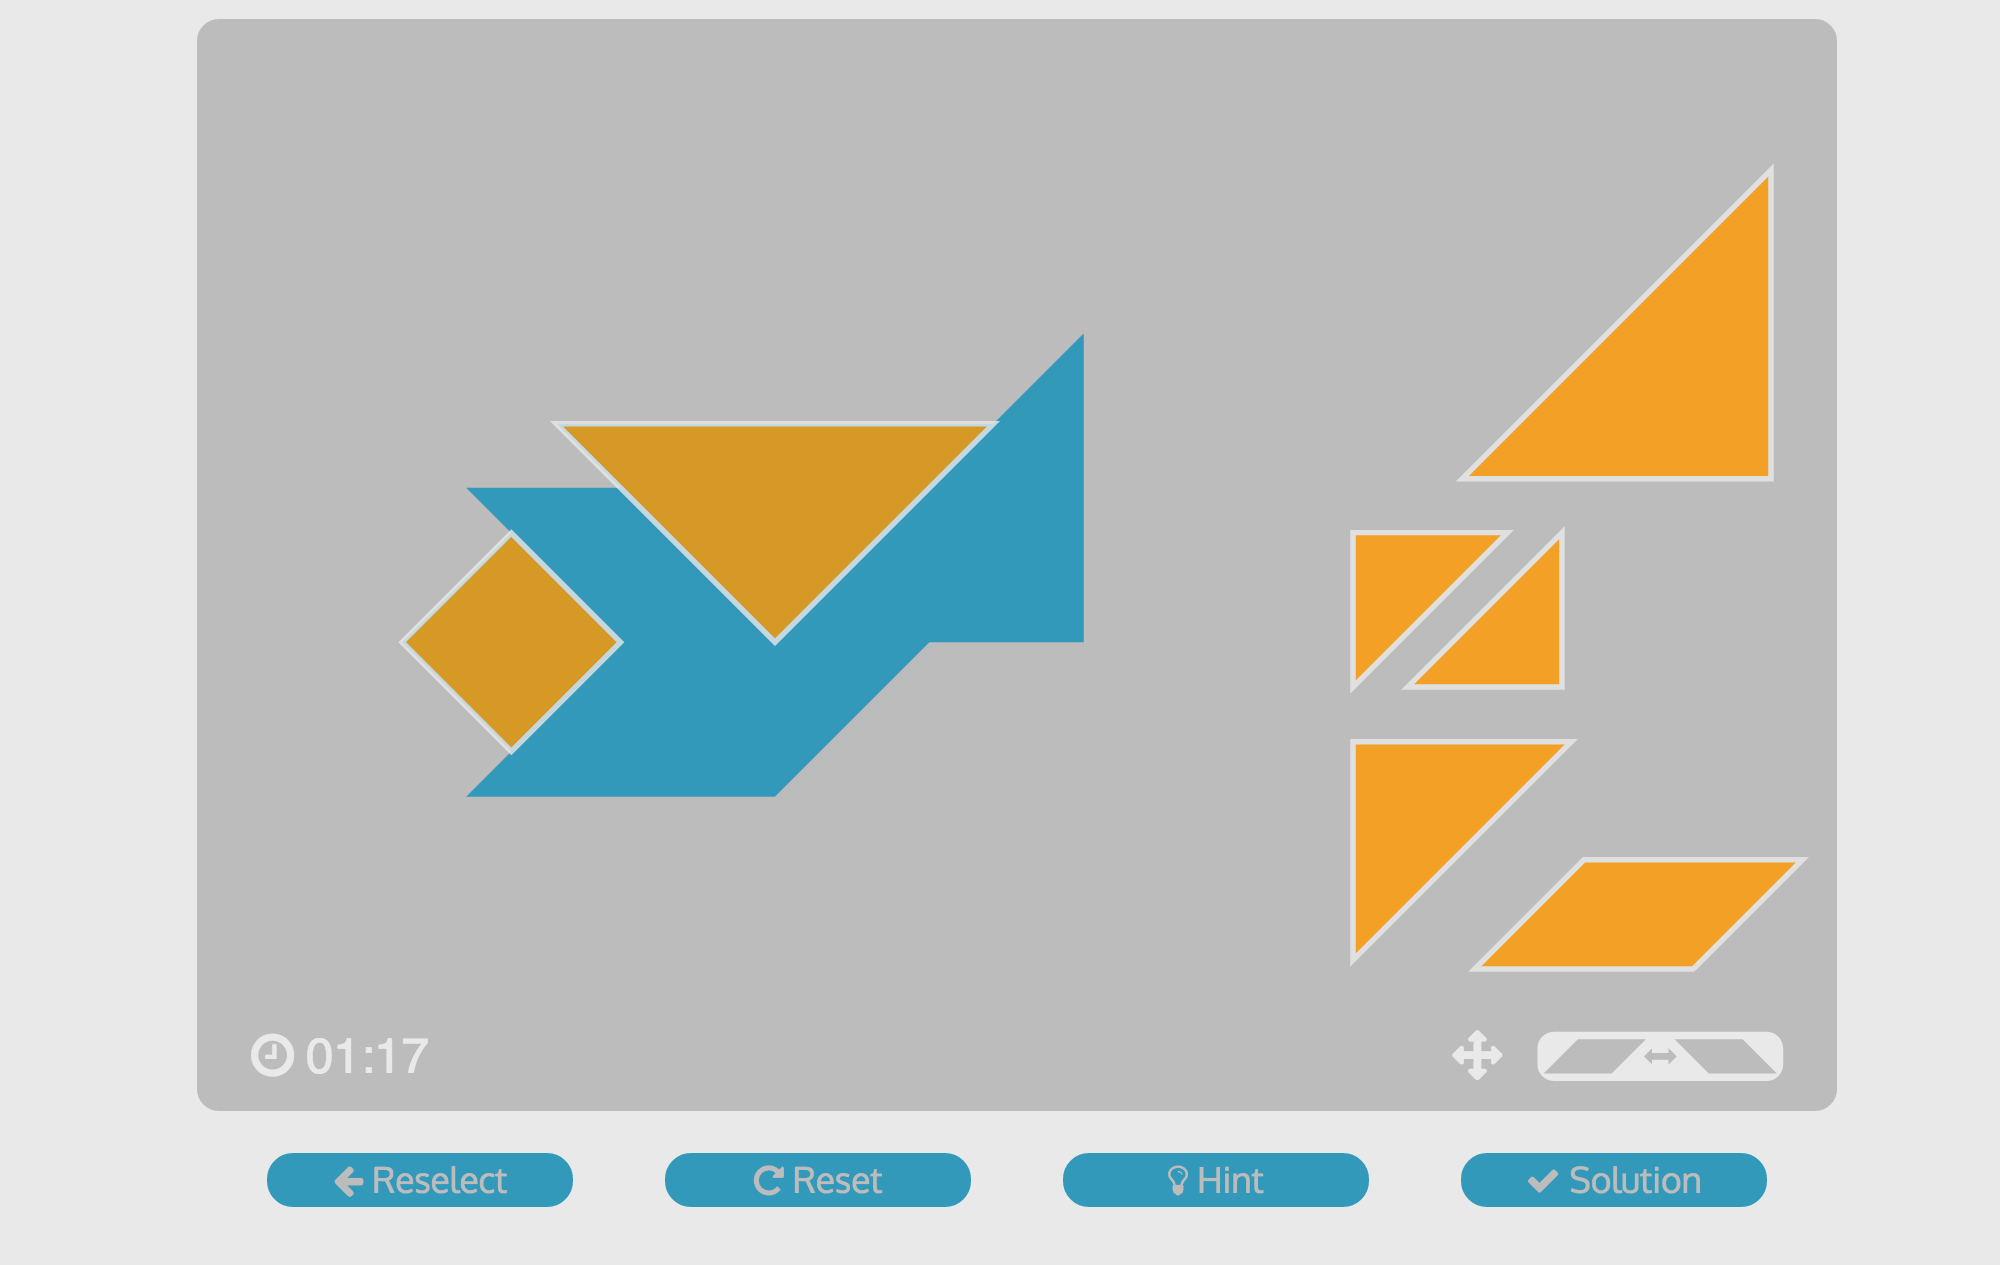
\includegraphics[width=0.9\textwidth]{figures/game.png}
  \caption{Interface allowing to solve a tangram}  
  \label{game}
\end{figure}

\section{Generation Process}
\label{generate}

Two approaches to randomly generate tangrams have been pursued. Both approaches have in common that they start out with generating an order for how the seven tans are placed and then position the first tangram. Subsequently new tans are placed by randomly choosing a vertex of one the already placed tans and choosing a vertex of the new tan. The new tan and the already places pieces are then connected at those two points if the placement of the new tan does not violate the constraint that pieces cannot overlap. A collection of invalid placements is shown in Figure \ref{figure}. If the placement fails, a new attempt of placing the tan is made. This process is continued until all 7 have been placed. 

%\missingfigure

Determining if a placement is valid is done in three steps. The first step uses the point-in-polygon algorithm mentioned before. All points of the newly placed tan as well as between one and four points inside the tan are tested for containment in other tans. The points inside of a tan are needed to correctly detect cases where one puzzle piece is entirely contained in another one. The direction vectors to these points are are pre-calculated and include vectors to the center of each tan and depending on the size of a tan more vectors that are derived from partitioning tans in some way. Without modification this would introduce thirds and halfs into coordinates, which is why the direction vectors of tangrams have been scaled by 6 compared to the dimensions presented in chapter \ref{chapter:background}. This still does not correctly handle cases where a large tan is placed on top of a small tan such that it lies completely inside the newly placed tan. Thus the same test is conducted the other way around. The second steps uses line segment intersection to determine of any of the segments of already placed tans intersect with the segments of a new tan.
Lastly, the bounding box of the tans including the newly placed tan is computed. The placement is then rejected if the the horizontal or vertical range is larger then a certain threshold. This step has been added in an attempt to avoid  sequences of tans that are only attached at one point and favour tangrams that are somewhat compact.

As a first naive approach an orientation for each tan is sampled at very beginning. The attachment point at the already placed tans is chosen first. Then all points of the new tan are considered as possible attachment points in random order. If none of the points can be used, a new attachment point of the placed tans is samples. Unfortunately, the fixed orientations together with the range threshold imposes a very strong restriction on the generation process which can lead to configurations where some tans are still missing, but cannot be placed anymore. Furthermore, this generation process leads to mostly loosely connected tangrams. Therefore, the second approach chooses orientations dynamically. Additionally, this approach steers the computation towards tangrams where tans have many edges in common.

The second approach starts out by sampling an orientation for the first tan and then places it. The process then continues to find two attachment points as before, however here, the orientation is sampled based on a probability distribution that favours orientations where the edges of the new tan align with already places pieces. This probability distribution is computed by checking if any of the segments meeting in the attachment point align for any of the orientations and apply a larger weight to such orientations. If the tan cannot be placed with the sampled orientation, a new orientation is sampled from the already computed probability distribution, where the probability of the just attempted orientation is set to zero. If none of the orientation lead to a valid placement, a new attachment point is chosen.

\section{Interestingness Measures}
\label{interesting}
convex hull

\section{Gameplay}
Outline computation \label{outline}

Snapping
